\section{Zoom agents}
\label{sec:agents}

\begin{figure*}[t]
\centering
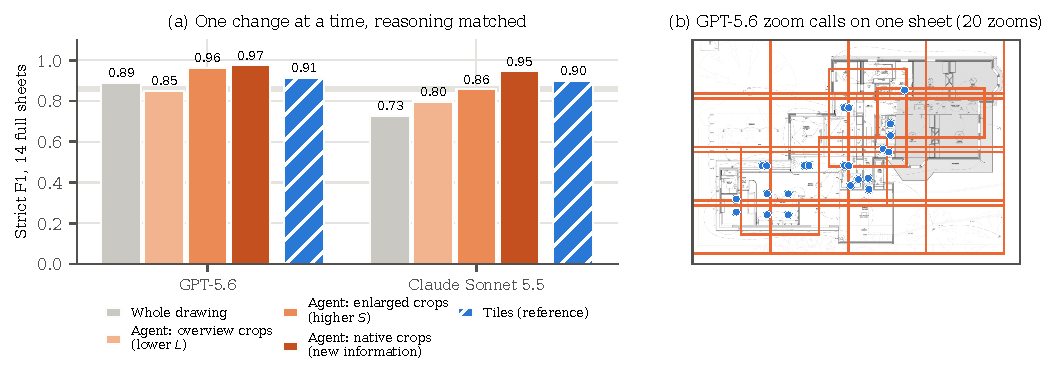
\includegraphics[width=\textwidth]{figures_x/fig_agent.pdf}
\caption{(a) F1 on the 14 full sheets with the same reasoning setting throughout (GPT-5.6: medium effort; Claude Sonnet 5.5: adaptive thinking). From left to right each bar changes one step: one whole-image call; an agent whose tool returns the requested region cut from the overview at the overview's scale (lower $L$ only); the same crops enlarged to the size of a native crop (also higher $S$, no new information); native crops (also new information); and, for reference, tiles. Agent bars average two runs, the overview-crop bars one. (b) The 20 regions GPT-5.6 chose on one sheet (orange), over the overview it received; blue dots are the annotated instances.}
\label{fig:agent}
\end{figure*}

\paragraph{Setup.} The agent receives the legend crop, an overview of the image (long side 1{,}600 px) and a \texttt{zoom} tool that returns any requested rectangle cut from the native image (long side at most 1{,}024 px, at most twice native), for up to 20 calls, with reasoning where the model has it (\cref{tab:models}). Each zoom raises $S$ by the enlargement factor and limits $L$ to the rectangle. Every image the agent keeps in its context is counted in its tokens, as in \cref{prop:frontier}.

\paragraph{Who splits, on the same model.} \Cref{tab:whosplits} puts side by side, for each model with an agent and with the same reasoning setting throughout, the whole-image call, the caller's split (tiles of the 44 px recipe, which zoom out on only one of these sheets) and the agent that splits the image itself. A model that zooms well can split more accurately than the caller's fixed tiles (GPT-5.6, Claude Sonnet 5.5); a model whose coordinates are unreliable across zoom levels fails when it splits itself (Gemini 3.8, Qwen3-VL). Only a caller's split that meets the condition, such as the rule, carries the protection of \cref{thm:exact} and a cost known before the call.

\begin{table}[t]
\centering
\small
\setlength{\tabcolsep}{3pt}
\resizebox{\columnwidth}{!}{\begin{tabular}{lccccc}
\toprule
 & \multicolumn{3}{c}{F1, 14 full sheets} & \multicolumn{2}{c}{Input tokens per drawing} \\
\cmidrule(lr){2-4}\cmidrule(lr){5-6}
Model & Whole & Caller's tiles & Agent & Tiles & Agent \\
\midrule
GPT-5.6 & \XnFAOneRgptFiveSixSheets & \XnFDRgptFiveSixSheets & \XnFAGgptFiveSixSheets & \XtileTokIngptFiveSix & \XagTokIngptFiveSix \\
Claude Sonnet 5.5 & \XnFAOneRsonnetFiveFiveSheets & \XnFDRsonnetFiveFiveSheets & \XnFAGsonnetFiveFiveSheets & \XtileTokInsonnetFiveFive & \XagTokInsonnetFiveFive \\
Gemini 3.8 & \XnFAOneRgemThreeEightSheets & \XnFDRgemThreeEightSheets & \XnFAGgemThreeEightSheets & \XtileTokIngemThreeEight & \XagTokIngemThreeEight \\
\bottomrule
\end{tabular}}
\caption{Who splits, on the same model and with the same reasoning setting (GPT-5.6: medium effort; Claude Sonnet 5.5: adaptive thinking; Gemini 3.8: dynamic thinking). Caller's tiles: the 44 px recipe and its fixed-grid counterpart, which zoom out on one of the 14 sheets for GPT-5.6 and Claude Sonnet 5.5 and on none for Gemini 3.8. Tokens: mean input tokens per LegendSpot test drawing. Qwen3-VL, which has no reasoning mode, reaches \XqD{} F1 with tiles and \XqAgF{} as an agent over all 34 drawings.}
\label{tab:whosplits}
\end{table}

\paragraph{Which step does the work.} \Cref{fig:agent}a changes one step at a time; the three steps are ordered by \cref{prop:zoom} at the level of single calls. Lowering $L$ alone gave no significant gain for either model (GPT-5.6 \XnHThreegptFiveSixOVCAOneR{} \XnHThreegptFiveSixOVCAOneRCI; Claude Sonnet 5.5 \XnHThreesonnetFiveFiveOVCAOneR{} \XnHThreesonnetFiveFiveOVCAOneRCI). Enlarging the same crops, which raises $S$ without new information, gave GPT-5.6 \XnHThreegptFiveSixOVZOVC{} \XnHThreegptFiveSixOVZOVCCI, and native pixels added \XnHThreegptFiveSixAGOVZ{} \XnHThreegptFiveSixAGOVZCI: for GPT-5.6 the active ingredient is $S$. For Claude Sonnet 5.5 no single step is decisive (enlargement \XnHThreesonnetFiveFiveOVZOVC{} \XnHThreesonnetFiveFiveOVZOVCCI), and only native pixels give a gain whose interval excludes zero (\XnHThreesonnetFiveFiveAGOVZ{} \XnHThreesonnetFiveFiveAGOVZCI): for it the overview lacks usable pixels, not only tokens~\cite{xu2020usable}. Over all 34 drawings the agents against their tiles differ by \XnAGDRallgptFiveSix{} \XnAGDRallgptFiveSixCI{} (GPT-5.6) and \XnAGDRallsonnetFiveFive{} \XnAGDRallsonnetFiveFiveCI{} (Claude Sonnet 5.5); on Library-10 GPT-5.6's agent again scores highest (\cref{tab:redp10}).

\paragraph{How the agents search.} GPT-5.6 used \XagZoomsgptFiveSix{} zooms per drawing on average; on several sheets it first laid a regular grid of equal crops over the whole image and then inspected candidate regions (\cref{fig:agent}b), and on full sheets it viewed \XagCovSheetsgptFiveSix{} of the area at $S \ge 1$. Claude Sonnet 5.5 used \XagZoomssonnetFiveFive{} zooms on average, none on 9 of the 20 small drawings, and concentrated them on hard sheets. The overview itself, at a median $S$ of \XovSmedSheets{} on full sheets, already covers much of each sheet. Per drawing, GPT-5.6's agent used \XagTokIngptFiveSix{} input and \XagTokOutgptFiveSix{} output tokens, against \XtileTokIngptFiveSix{} and \XtileTokOutgptFiveSix{} for its tiles; Claude's agent used \XagTokInsonnetFiveFive{} and \XagTokOutsonnetFiveFive, about half of its tiles (\XtileTokInsonnetFiveFive{} and \XtileTokOutsonnetFiveFive). On floor-plan mosaics, where the first block's content is fixed while the mosaic grows, GPT-5.6's agent stays flat in first-block F1, as tiles do and whole-image calls do not (\cref{sec:firstblock}).

\paragraph{Two agents fail at the coordinates.} The Gemini 3.8 and Qwen3-VL agents count about as well as their tiles but place points wrongly. Gemini 3.8 used the most zooms (\XagZoomsgemThreeEight, \XagTokIngemThreeEight{} input tokens per drawing) and scored \XagFgemThreeEightAll{} F1 (against its tiles \XagMinusDgemThreeEight{} \XagMinusDCIgemThreeEight), yet gave the exact count on \XagExactCountgemThreeEight\% of drawings. Qwen3-VL scored \XqAgF, against \XqD{} for its tiles (\XqAgMinusD{} \XqAgMinusDCI), with a median relative count error of \XqCountErrAg, no worse than with tiles (\XqCountErrD). A check on the stored trajectories, with no new call, locates the failure. The count is within 10\% of the truth on \CagCntGem\% of the drawings for the Gemini 3.8 agent (\CtileCntGem\% for its tiles) and on \CagCntQwen\% for the Qwen3-VL agent (\CtileCntQwen\%). The points are not: \CagLocGem\% of the Gemini 3.8 agent's points lie within $\tau$ of an instance and \CagLocGemTwo\% within $2\tau$ (median distance to the nearest instance \CagDistGem$\,\tau$), against \CtileLocGem\% for its tiles; for Qwen3-VL, \CagLocQwen\% and \CagLocQwenTwo\% (median \CagDistQwen$\,\tau$), against \CtileLocQwen\%. Reading the agents' answers in the other coordinate convention makes them worse, so the convention is not the cause. Agents and tiles both see crops of native pixels; what differs is that the agent itself converts positions seen in a zoomed crop back to the overview, a conversion that no tiled or whole-image call requires (\cref{sec:coords}).
